% !TEX root = main.tex

\section{Compiler organization}


\begin{frame}{Compiler pipeline}
\begin{center}
Typically a compiler is a \alert{pipeline}.\\
\bigskip
Advantages of the pipeline model:\\
\medskip
\begin{varwidth}{0.8\textwidth}
\begin{itemize}
\item \alert{simplicity} -- read something, produce something
\item \alert{locality} -- no superfluous state
\end{itemize}
\end{varwidth}
\\
\bigskip
Complexity lies on \alert{chaining} together stages.
\end{center}
\end{frame}


\begin{frame}{Compiler pipeline}{Internal pipelines}
\begin{center}
High-level pipeline structure of a compiler:\\
\begin{figure}
\centering

% compiler-structure.tex: generic organization of a compiler.

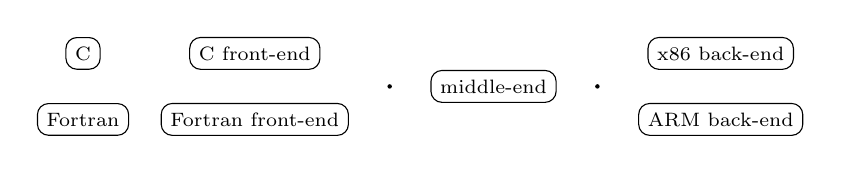
\begin{tikzpicture}
[
  every node/.style={
    font=\scriptsize
  },
  cell/.style={
    rectangle,
    rounded corners,
    draw
  },
  point/.style={
    circle,
    fill,
    inner sep=.2mm
  },
  tip/.style={
    ->,
    shorten >=.5mm,
    shorten <=.5mm
  },
  man-tip/.style={
    tip,
    to path={-| (\tikztotarget)}
  },
  rman-tip/.style={
    tip,
    to path={|- (\tikztotarget)}
  }
]

\matrix [column sep=4mm]
{
\node (c-language)   [cell] {C};             &
\node (c-front-end)  [cell] {C front-end};   &
\node ()             []     {};              &
\node ()             []     {};              &
\node ()             []     {};              &
\node (x86-back-end) [cell] {x86 back-end}; \\

\node ()               []      {};           &
\node ()               []      {};           &
\node (middle-end-in)  [point] {};           &
\node (middle-end)     [cell]  {middle-end}; &
\node (middle-end-out) [point] {};           &
\node ()               []      {};          \\

\node (fortran-language)  [cell] {Fortran};           &
\node (fortran-front-end) [cell] {Fortran front-end}; &
\node ()                  []     {};                  &
\node ()                  []     {};                  &
\node ()                  []     {};                  &
\node (arm-back-end)      [cell] {ARM back-end};     \\
};

{ [start chain]
\chainin (c-language)    [join];
\chainin (c-front-end)   [join=by tip];
\chainin (middle-end-in) [join=by man-tip];
}

{ [start chain]
\chainin (fortran-language)  [join];
\chainin (fortran-front-end) [join=by tip];
\chainin (middle-end-in)     [join=by man-tip];
}

{ [start chain]
\chainin (middle-end-in)  [join];
\chainin (middle-end)     [join=by tip];
\chainin (middle-end-out) [join=by tip];
}

{ [start chain]
\chainin (middle-end-out) [join];
\chainin (x86-back-end)   [join=by rman-tip];
}

{ [start chain]
\chainin (middle-end-out) [join];
\chainin (arm-back-end)   [join=by rman-tip];
}
\end{tikzpicture}

\end{figure}
\medskip
There are three main components:

\begin{description}
\item[Front-end] \alert{translate} a source file into the intermediate representation
\item[Middle-end] \alert{analyze} the intermediate representation, \alert{optimize}
                  it
\item[Back-end] \alert{generate} target machine assembly from the intermediate
                representation
\end{description}
\end{center}
\end{frame}


\begin{frame}{The LLVM compiler pipeline}
\begin{center}
We will consider only the \emph{middle-end}.\\
{\small Same concepts are valid also for \{front,back\}-end.}\\
\bigskip
\begin{description}[Pass Manager]
\item[IR] (a.k.a. Intermediate Representation) the \alert{language} used in the
          middle-end
\item[Pass] a \alert{pipeline stage}\\
a Pass may have \alert{dependencies} on other Passes.
\item[Pass Manager] component that \alert{schedules} passes according to their \alert{dependencies} and \alert{executes} them\\
\emph{(builds the pipeline)}
\end{description}
\end{center}
\end{frame}


\begin{frame}{First insights}
A compiler is \alert{complex}:

\begin{itemize}
\item passes are the \alert{elementary unit of work}
\item Pass Manager must be \alert{advised} about pass chaining
\item pipeline shapes are \alert{not fixed} -- they can change from one compiler
      execution to another\\
      {\small e.g. optimized/not optimized builds, compiler options, ...}
\end{itemize}
\end{frame}


\begin{frame}{A word of warning!}
\begin{center}
{\large 
Compilers must be \alert{conservative}:\\
\smallskip
$\Downarrow$\\
\smallskip
All passes \alert{must preserve the program semantics}\\
\smallskip
$\Downarrow$\\
\smallskip
Compiler passes must be designed \alert{very carefully}!\\
}
\end{center}
\end{frame}
